\documentclass[10pt,a4paper,fleqn,landscape]{article}
\usepackage[ngerman]{babel}
\usepackage[utf8]{inputenc}
\usepackage[T1]{fontenc}

\usepackage[landscape]{geometry}
\usepackage{multicol}
% for landscape format: insert "landscape" at documentclass and geometry

\usepackage{float}
\usepackage{graphicx}
\usepackage{amsmath, amsfonts, amssymb,esint}
\usepackage{trfsigns}
\usepackage{bm}
\usepackage{empheq}
\usepackage{siunitx}

\geometry{top=0.5cm,left=1cm,right=1cm,bottom=0.5cm}

\setlength{\mathindent}{0mm}
\setlength{\parindent}{0mm}
\setlength{\parskip}{0mm}
\setlength{\jot}{5pt}
\setlength{\abovedisplayskip}{0pt}
\setlength{\belowdisplayskip}{5pt}
\setlength{\abovedisplayshortskip}{0pt}
\setlength{\belowdisplayshortskip}{5pt}

\setlength{\columnseprule}{0.25pt}
\setlength{\premulticols}{1pt}
\setlength{\postmulticols}{1pt}
\setlength{\multicolsep}{1pt}
\setlength{\columnsep}{10pt}


\makeatletter
\renewcommand{\section}{\@startsection{section}{1}{0mm}%
                                {-1ex plus -.5ex minus -.2ex}%
                                {0.5ex plus .2ex}%x
                                {\normalfont\large\bfseries}}
\renewcommand{\subsection}{\@startsection{subsection}{2}{0mm}%
                                {-1explus -.5ex minus -.2ex}%
                                {0.5ex plus .2ex}%
                                {\normalfont\normalsize\bfseries}}
\renewcommand{\subsubsection}{\@startsection{subsubsection}{3}{0mm}%
                                {-1ex plus -.5ex minus -.2ex}%
                                {1ex plus .2ex}%
                                {\normalfont\small\bfseries}}

\g@addto@macro\normalsize{	% adapt if changing fontsize
  \setlength\abovedisplayskip{5pt}
  \setlength\belowdisplayskip{5pt}
  \setlength\abovedisplayshortskip{5pt}
  \setlength\belowdisplayshortskip{5pt}
}                   
                                
\makeatother
\setcounter{secnumdepth}{0}

% Command Defs ------------------------------------------------------------------------------------------------

\newcommand{\HL}{\rule{\linewidth}{0.25pt}}		% Command for horizontal separation line
\newcommand{\EW}{\mathbb{E}}
\newcommand{\vc}[1]{\vec{\underline{#1}}} 		% <-- Use this shit for komplex vectors: 	example: \vc{H}
\renewcommand{\c}[1]{\underline{#1}}			% <-- Use this shit für komplexe scalars: 	example: \c{H}_x
\renewcommand{\j}{{\mathrm j}}					% imaginary unit
\newcommand{\D}{{\mathrm d}}					% differential d for dx and stuff
\newcommand{\matr}[1]{\bm{#1}}				% <-- use this shit for ISO-complying matrix notation
\newcommand{\norm}[1]{\left\lVert#1\right\rVert}	% <-- because abs are to mainstream
%-------------------------------------------------------------------------------------------------------------

\pagestyle{empty}

\begin{document}
	
%\small
\begin{multicols}{2}
\section{Grundlagen}
\subsection{Zeitharmonische Maxwell-Gleichungen}
für anisotrope, homogene Medien
	\begin{align*}
	\nabla\times\vc{H} &= \vc{J} + \j\omega\varepsilon\vc{E} &\iff&& \oint_{\partial A}\vc{H}\cdot\D\vec{s} &= \iint_A\left( \vc{J} + \j\omega\varepsilon\vc{E}\right) \cdot\D\vec{A}\\
	-\nabla\times\vc{E} &= \vc{M} + \j\omega\mu\vc{H} &\iff&& -\oint_{\partial A}\vc{E}\cdot\D\vec{s} &= \iint_A\left( \vc{M} + \j\omega\mu\vc{H}\right) \cdot\D\vec{A}\\
	\nabla\cdot\vc{H}&=\c{\rho}_m/\mu &\iff&& \varoiint_{\partial V}\vc{H}\cdot\D\vec{A}&=\frac{1}{\mu}\iiint_V \c{\rho}_m\D V\\
	\nabla\cdot\vc{E}&=\c{\rho}_e/\varepsilon &\iff&& \varoiint_{\partial V}\vc{E}\cdot\D\vec{A}&=\frac{1}{\varepsilon}\iiint_V \c{\rho}_e\D V
	\end{align*}
für Freiraumausbreitung und allgemein Vakuum: $\c{\rho}_e=\c{\rho}_m=0$ und $\vc{J}=\vc{M}=\vec{0}$

\subsection{Poynting-Vektor; Wirkleistung}
	\begin{equation*}
	\vc{S}=\frac{1}{2}\vc{E}\times\vc{H}^*\quad;\quad P=\varoiint\Re\left\lbrace \vc{S} \right\rbrace \D\vec{A} =\frac{1}{2}\varoiint\Re\left\lbrace \vc{E}\times\vc{H}^* \right\rbrace \D\vec{A}
	\end{equation*}
\subsection{Berechnung der Transversal- aus den Longitudinalkomponenten}
	\begin{align*}
		\c{E}_\text{x}\beta_\text{c}^2&=\mp\j\beta\frac{\partial\c{E}_\text{z}}{\partial x}-\j\omega\mu\frac{\partial\c{H}_\text{z}}{\partial y} & \c{E}_\text{y}\beta_\text{c}^2&=\mp\j\beta\frac{\partial\c{E}_\text{z}}{\partial y}+\j\omega\mu\frac{\partial\c{H}_\text{z}}{\partial x}\\
		\c{H}_\text{x}\beta_\text{c}^2&=\mp\j\beta\frac{\partial\c{H}_\text{z}}{\partial x}+\j\omega\varepsilon\frac{\partial\c{E}_\text{z}}{\partial y} & \c{H}_\text{y}\beta_\text{c}^2&=\mp\j\beta\frac{\partial\c{H}_\text{z}}{\partial y}-\j\omega\varepsilon\frac{\partial\c{E}_\text{z}}{\partial x}
	\end{align*}
\HL
\section{Polarisation}
\subsection{Drehsinn und Form}
\begin{itemize}
	\item $\SI{0}{\degree}<\alpha_\text{x}-\alpha_\text{y}<\SI{180}{\degree}$ : $E_{0\text{x}}$ eilt $E_{0\text{y}}$ vor, rechtsdrehend
	\item $\SI{0}{\degree}<\alpha_\text{y}-\alpha_\text{x}<\SI{180}{\degree}$ : $E_{0\text{y}}$ eilt $E_{0\text{x}}$ vor, linksdrehend
	\item $\alpha_\text{x}-\alpha_\text{y}=\SI{0}{\degree}$ oder $\alpha_\text{x}-\alpha_\text{y}=\SI{180}{\degree}$ : $E_{0\text{x}}$ oder $E_{0\text{y}}$ gleich- oder gegenphasig, linear
	\item $\alpha_\text{x}-\alpha_\text{y}=\SI{90}{\degree}$ und $|\c{E}_{0\text{x}}|=|\c{E}_{0\text{y}}|$ : rechtsdrehend, zirkular
	\item $\alpha_\text{y}-\alpha_\text{x}=\SI{90}{\degree}$ und $|\c{E}_{0\text{x}}|=|\c{E}_{0\text{y}}|$ : linksdrehend, zirkular
\end{itemize}
\subsection{HowTo: zeichnen einer Polarisationsellipse}
\begin{enumerate}
	\item Realteile der komplexen Amplituden
		\begin{align*}
			E_{0\text{x}}&=\Re{\left\{ \c{E}_{0\text{x}}e^{\j\omega t}\right\}} = A\cos(\omega t) - B\sin(\omega t) \\
			E_{0\text{y}}&=\Re{\left\{ \c{E}_{0\text{y}}e^{\j\omega t}\right\}} = C\cos(\omega t) - D\sin(\omega t)
		\end{align*}
	\item Maximalwerte der Komponenten berechnen
		\begin{align*}
			E_{0\text{x,max}}&=|E_{0\text{x}}|=\sqrt{A^2+B^2}\\
			E_{0\text{y,max}}&=|E_{0\text{y}}|=\sqrt{C^2+D^2}
		\end{align*}
	\item Betrag des Ellipsenradius
		\begin{align*}
			&\norm{\vec{E}_0}=\sqrt{E^2_{0\text{x}}+E^2_{0\text{y}}}=\sqrt{A_0+A_1\cos(2\omega t)-A_2\sin(2\omega t)}\\
			&=\sqrt{\frac{A^2+B^2+C^2+D^2}{2}+\frac{A^2-B^2+C^2-D^2}{2}\cos(2\omega t)-(AB+CD)\sin(2\omega t)}
		\end{align*}
	\item Umformen des hinteren Ausdrucks
		\begin{align*}
			A_1\cos(2\omega t)-A_2\sin(2\omega t)&=\Re\left\{(A_1+jA_2)e^{\j2\omega t}\right\}\\
			&=\sqrt{A_1^2+A_2^2}\cos\left(2\omega t+\arctan\left(\frac{A_2}{A_1}\right)\right)
		\end{align*}
	\item maximale und minimale Amplitude
		\begin{equation*}
			E_{^\text{max}_\text{min}}=\sqrt{A_0\pm\sqrt{A_1^2+A_2^2}}
		\end{equation*}
	\item Berechnung der Zeitpunkte aus der Phase
		\begin{equation*}
			2\omega t_{^\text{max}_\text{min}}+\arctan\left(\frac{A_2}{A_1}\right)=
			\begin{matrix}
				0\\
				+\pi
			\end{matrix}
		\end{equation*}
	\item Winkel der maximalen und Minimalen Amplituden
		\begin{equation*}
			\tan(\alpha)=\frac{E_{0\text{y}}\left(t_{\text{max}}\right)}{E_{0\text{x}}\left(t_{\text{max}}\right)}=\frac{C\cos\left(\omega t_{\text{max}}\right)-D\sin\left(\omega t_{\text{max}}\right)}{A\cos\left(\omega t_{\text{max}}\right)-B\sin\left(\omega t_{\text{max}}\right)}
		\end{equation*}
	\item Ellipse zeichnen

		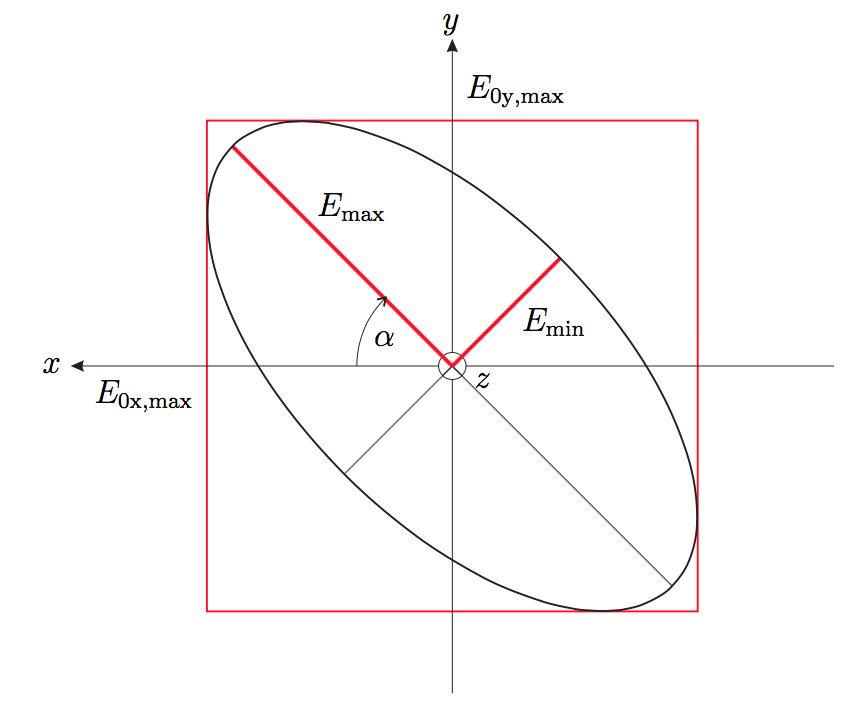
\includegraphics[width=0.6\linewidth]{img/polarisationsellipse}
\end{enumerate}
\HL
\section{EM-Wellen: allgemeine Zusammenhänge}
\subsection*{Wellenleiter (konstanter Querschnitt)}
	\begin{equation*}
		\lambda=\frac{\lambda_0}{\sqrt{1-\left(\frac{\beta_\text{c}}{\beta_0 }\right)^2 }}=\frac{\lambda_0}{\sqrt{1-\left(\frac{f_\text{c}}{f}\right)^2 }}=\frac{\lambda_0}{\sqrt{1-\left(\frac{\lambda_0}{\lambda_\text{c}}\right)^2 }}
	\end{equation*}
	
	Phasengeschwindigkeit
	\begin{equation*}
		v_{\text{p}}=\frac{c}{\sqrt{1-\left(\frac{\beta_\text{c}}{\beta_0}\right)^2}}=\frac{c}{\sqrt{1-\left(\frac{f_\text{c}}{f}\right)^2}}=\frac{c}{\sqrt{1-\left(\frac{\lambda_0}{\lambda_\text{c}}\right)^2}}
	\end{equation*}
	
	Gruppengeschwindigkeit
	\begin{equation*}
		v_{\text{g}}=c\sqrt{1-\left(\frac{\beta_\text{c}}{\beta_0}\right)^2}=c\sqrt{1-\left(\frac{f_\text{c}}{f}\right)^2}=c\sqrt{1-\left(\frac{\lambda_0}{\lambda_\text{c}}\right)^2}
	\end{equation*}
	
	Zusammenhang Geschwindigkeiten
	\begin{equation*}
		c_0^2=v_\text{g}\cdot v_\text{p}
	\end{equation*}
	
	Kritische Frequenzen ($a>b$)
	\begin{equation*}
		f_{\text{c},m,n} = \frac{c}{2}\cdot\sqrt{\left(\frac{m}{a}\right)^2+\left(\frac{n}{b}\right)^2}	\qquad f_\text{c}=\frac{\beta_\text{c}}{2\pi\sqrt{\varepsilon\mu}}=\frac{f_{\text{c}0}}{\sqrt{\varepsilon_r\mu_r}} \qquad \beta^2_\text{c}=\beta^2_0-\beta^2
	\end{equation*}
\subsection*{Zweileitersysteme}
Gruppen- und Phasengeschwindigkeit
	\begin{equation*}
		v_\text{g}=v_\text{p}=\frac{1}{\sqrt{\varepsilon\mu}}=\frac{1}{\sqrt{L'C'}}=c
	\end{equation*}
Leitungsbeläge Koaxialleitung
	\begin{equation*}
		C' = \frac{C}{l} = \frac{2\pi\varepsilon}{\ln\left(\frac{D}{d}\right)} \qquad L' = \frac{\varepsilon\mu}{C'} = \frac{\mu\ln\left(\frac{D}{d}\right)}{2\pi}
	\end{equation*}
Wellenwiderstand
	\begin{equation*}
		\pm Z_\text{L}=\frac{\c{U}(z)}{\c{I}(z)}=\frac{\c{U}_0}{\c{I}_0}
	\end{equation*}
\subsection{Koaxialleitung}
	Wellenwiderstand und Leistung
	\begin{equation*}
		Z_\text{L}=\frac{1}{2\pi}Z_{\text{F}0}\ln\left(\frac{D}{d}\right) \qquad P=\frac{1}{2}Z_\text{L}I^2_{\text{max}}=\frac{1}{2}\frac{U^2_{\text{max}}}{Z_\text{L}}=\frac{1}{2}\int\limits^{2\pi}_0 \int\limits^D_d \frac{E(r)^2}{Z_\text{F}}\D A
	\end{equation*}
	Feldstärken
	\begin{equation*}
		H_\text{max}=\frac{I_\text{max}}{\pi d} \qquad E_\text{max}=Z_\text{F}H_\text{max}
	\end{equation*}
	Strahlungsleistungsdichten Innen- und Außenleiter
	\begin{equation*}
		S_\text{I}=\frac{1}{2}E_\text{max}\cdot H_\text{max} \qquad S_\text{A}=S_\text{I}\frac{d^2}{D^2}
	\end{equation*}
	
\subsection*{Feldwellenwiderstand}
TE-Wellen
	\begin{align*}
		Z_\text{FH} &= \pm\frac{\vc{E}_\text{x}}{\vc{H}_\text{y}} = \mp\frac{\vc{E}_\text{y}}{\vc{H}_\text{x}}\\
		&= \frac{\omega\mu}{\beta} = \frac{\omega\mu}{\beta_0\sqrt{1-\left(\frac{\beta_\text{c}}{\beta_0}\right)^2}} = \frac{Z_\text{F}}{\sqrt{1-\left(\frac{\beta_\text{c}}{\beta_0}\right)^2}} = \frac{Z_\text{F}}{\sqrt{1-\left(\frac{f_\text{c}}{f_0}\right)^2}} = \frac{Z_\text{F}}{\sqrt{1-\left(\frac{\lambda_0}{\lambda_\text{c}}\right)^2}}
	\end{align*}
TM-Wellen
	\begin{align*}
		Z_\text{FE} &= \pm\frac{\vc{E}_\text{x}}{\vc{H}_\text{y}} = \mp\frac{\vc{E}_\text{y}}{\vc{H}_\text{x}} = \frac{\beta}{\omega\varepsilon} = \frac{\beta_0\sqrt{1-\left(\frac{\beta_\text{c}}{\beta_0}\right)^2}}{\omega\varepsilon} \\
		&= Z_\text{F} \sqrt{1-\left(\frac{\beta_\text{c}}{\beta_0}\right)^2} = Z_\text{F} \sqrt{1-\left(\frac{f_\text{c}}{f_0}\right)^2} = Z_\text{F} \sqrt{1-\left(\frac{\lambda_0}{\lambda_\text{c}}\right)^2}
	\end{align*}
TEM-Wellen
	\begin{equation*}
		\frac{\vc{E}_\text{x}}{\vc{H}_\text{y}} = -\frac{\vc{E}_\text{y}}{\vc{H}_\text{x}} = \pm\frac{\omega\mu}{\beta} = \pm\sqrt{\frac{\mu}{\varepsilon}} = \pm Z_F \qquad Z_{\text{F}0} = \sqrt{\frac{\mu_0}{\varepsilon_0}} = 120\pi\Omega = 377\Omega
	\end{equation*}
\HL
\section{Antennentheorie}
\subsection{Feldgrößen}
Vektorpotential Fernfeldnäherung
	\begin{equation*}
		\vc{A}(\vec{r})=\frac{\mu e^{-\j\beta r}}{4\pi r}\iiint\limits_V\vc{J}e^{\j\beta r' \cos(\xi)}\D V'
	\end{equation*}
Feldstärken
	\begin{equation*}
		\vc{B}\approx-\j\beta\vec{u}_r\times\vc{A} \qquad \vc{H}\approx-\frac{\j\beta}{\mu}\vec{u}_r\times\vc{A} \qquad \vc{E}\approx\j\omega\times(\vec{u}_r\times\vc{A})
	\end{equation*}
\subsection{Kenngrößen von Antennen}
Strahlungsleistungsdichte (Allgemeine/Kugel/Dipol)
	\begin{equation*}
		S=\frac{P\cdot G	}{4\pi r^2} \qquad S_0=\frac{P}{4\pi r^2} \qquad S(\vartheta,\varphi)=\frac{1}{2}Z_\text{F}\left(\frac{\beta|\c{I}_0|l\sin(\vartheta)}{4\pi r}\right)^2 \sim \frac{1}{r^2}
	\end{equation*}
Richtfaktor
	\begin{equation*}
		D=\frac{S_{\text{max}}}{S_0}	=\frac{S_{\text{max}}}{P}\cdot4\pi r^2 \qquad \text{bzw.} \qquad D(\vartheta,\varphi)=\frac{S(\vartheta,\varphi)}{S_0}
	\end{equation*}
	\begin{empheq}[box=\fbox]{equation*}
		D_{Kugel}=\frac{S_0}{S_0}=1	
	\end{empheq}

Gewinn und Zusammenhang mit Wirkfläche für alle Antennen
	\begin{equation*}
		G=\eta D \qquad \frac{A}{G}=\frac{\lambda^2}{4\pi}
	\end{equation*}
Richcharakteristik
	\begin{equation*}
		C(\vartheta,\varphi)=\frac{\left\Vert\vc{E}(\vartheta,\varphi)\right\Vert}{\left\Vert\vc{E}\right\Vert_\text{max}}=\frac{\left\Vert\vc{H}(\vartheta,\varphi)\right\Vert}{\left\Vert\vc{H}\right\Vert_\text{max}}=\sqrt{\frac{S(\vartheta,\varphi)}{S_\text{max}}}
	\end{equation*}
Abgestrahlte Leistung
	\begin{equation*}
		P=\varoiint S\D A = \varoiint S_0DC^2(\vartheta,\varphi)\D A
	\end{equation*}
Empfangene Leistung
	\begin{equation*}
		P_\text{E}=S\cdot A_\text{E}
	\end{equation*}
Fußpunktimpedanz und Strahlungswiderstand
	\begin{equation*}
		\c{Z}_\text{A}=\frac{\c{U}_0}{\c{I}_0} \qquad R_\text{S}=\frac{2P}{|\c{I}_0|^2}
	\end{equation*}
\HL
\section{Reflexion}
\subsection{Abstandsabhängige komplexe Wellenamplituden}
	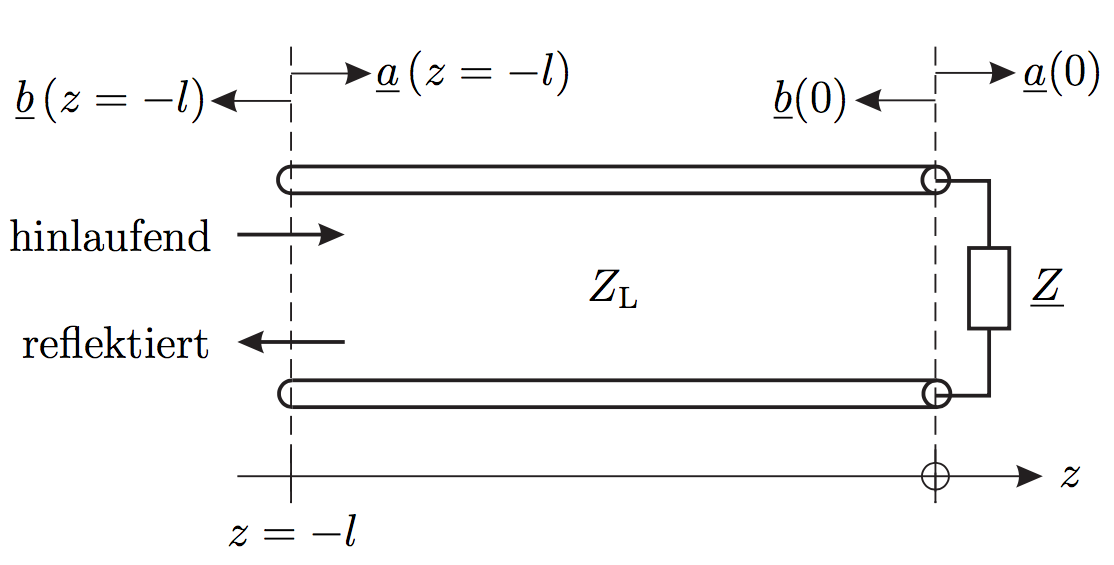
\includegraphics[width=0.5\linewidth]{img/wellenleiter}
	\begin{align*}
		\c{a}(z)&=\c{a}_0(z)e^{-\j\beta z} & \c{\Gamma}_0&=\frac{\c{b}_0}{\c{a}_0}=\frac{\c{Z}-\c{Z}_\text{L}}{\c{Z}+\c{Z}_\text{L}}=\c{\Gamma}(z=0)\\
		\c{b}(z)&=\c{b}_0(z)e^{+\j\beta z} & \c{\Gamma}(z)&=\frac{\c{b}(z)}{\c{a}(z)}=\frac{\c{b}_0e^{+\j\beta z}}{\c{a}_0e^{-\j\beta z}}=\c{\Gamma}_0e^{+\j2\beta z}\\
	\end{align*}
	Wenn $z=0$ am Anfang des Leiters muss die Phase von $\c{\Gamma}_0$ zurückgedreht werden. Es gilt (Bsp.):
	\begin{equation*}
		\c{\Gamma}_0=\frac{\c{Z}-\c{Z}_\text{L}}{\c{Z}+\c{Z}_\text{L}}e^{-\j2\beta l}
	\end{equation*}
	$U(z)$ und $I(z)$ können so berechnet werden wie an einem Tor eines Zweitores. Dafür Ausdruck so umformen, dass Abhängigkeit nur noch von $\c{a}$
	\begin{equation*}
		\c{a}(z)=\frac{\c{U}(z)}{\sqrt{\c{Z}_\text{L}}}=\pm \sqrt{\c{Z}_\text{L}}\c{I}(z) \qquad \c{c}(z)=\c{a}(z)+\c{b}(z)
	\end{equation*}
\HL
\section{Zweitore}
\subsection{Wellengrößen}
	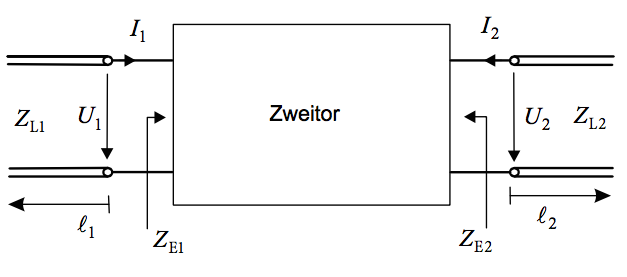
\includegraphics[width=0.5\linewidth]{img/zweitor1}
	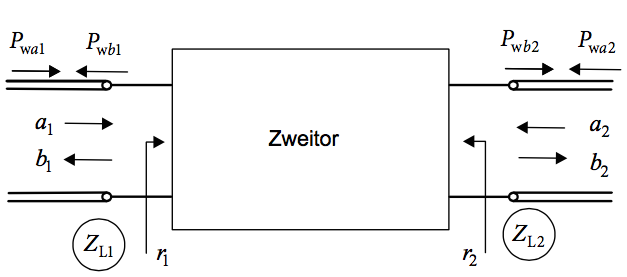
\includegraphics[width=0.5\linewidth]{img/zweitor2}
	
Komplexe Wellenamplituden
	\begin{align*}
		\c{a}_i&=\frac{\c{U}_{\text{h}i}}{\sqrt{\c{Z}_{\text{L}_i}}} \qquad \text{(hinlaufenden normierte Spannungswelle an Tor $i$)}\\
		\c{b}_i&=\frac{\c{U}_{\text{r}i}}{\sqrt{\c{Z}_{\text{L}i}}} \qquad \text{(rücklaufende normierte Spannungswelle an Tor $i$)}
	\end{align*}
Spannung und Strom an Tor $i$
	\begin{align*}
		\c{U}_i&=(\c{a}_i+\c{b}_i)\sqrt{\c{Z}_{\text{L}i}} & \c{a}_i&=\frac{\c{U}_i+\c{Z}_{\text{L}i}\c{I}_i}{2\sqrt{\c{Z}_{\text{L}i}}} \\
		\c{I}_i&=\frac{\c{a}_i-\c{b}_i}{\sqrt{\c{Z}_{\text{L}i}}} & \c{b}_i&=\frac{\c{U}_i-\c{Z}_{\text{L}i}I_i}{2\sqrt{\c{Z}_{\text{L}i}}}
	\end{align*}
Wirkleistung
	\begin{equation*}
		P_{\text{w}ai}=\frac{1}{2}\c{a}_i\c{a}_i^*=\frac{\c{U}_{\text{h}i}\c{U}_{\text{h}i}^*}{2\c{Z}_{\text{L}i}}=\frac{1}{2}|\c{a}_i|^2 \qquad P_{\text{w}bi}=\frac{1}{2}\c{b}_i\c{b}_i^*=\frac{\c{U}_{\text{r}i}\c{U}_{\text{r}i}^*}{2\c{Z}_{\text{L}i}}=\frac{1}{2}|\c{b}_i|^2
	\end{equation*}
\subsection{Matrizen}
Streumatrix
	\begin{equation*}
		\c{\matr{b}} = \c{\matr{S}}\cdot\c{\matr{a}}
	\end{equation*}
	\begin{equation*}
		\c{\matr{S}}^{\ast\text{T}}\cdot\c{\matr{S}}=\matr{E} \qquad \text{Unitaritätskriterium, Vorraussetzung für Verlustfreiheit}
	\end{equation*}
Transmissionsmatrix
	\begin{align*}
		\begin{pmatrix}
			\c{a}_1\\
			\c{b}_1
		\end{pmatrix}
		&=
		\begin{pmatrix}
			\c{T}_{11} & \c{T}_{12}\\
			\c{T}_{21} & \c{T}_{22}	
		\end{pmatrix}
		\cdot
		\begin{pmatrix}
			\c{b}_2\\
			\c{a}_2
		\end{pmatrix}\\
		\c{\matr{T}} &= \frac{1}{\c{S}_{21}}\cdot
		\begin{pmatrix}
			1 & -\c{S}_{22}\\
			\c{S}_{11} & -\det(\c{\matr{S}})
		\end{pmatrix} \qquad
		\c{\matr{S}} = \frac{1}{\c{T}_{11}}\cdot
		\begin{pmatrix}
			\c{T}_{21} & \det(\c{\matr{T}})\\
			1 & -\c{T}_{12}
		\end{pmatrix}
	\end{align*}
Kettenmatrix
	\begin{equation*}
		\begin{pmatrix}
			\c{U}_1\\
			\c{I}_1
		\end{pmatrix}
		=
		\begin{pmatrix}
			\c{A} & \c{B}\\
			\c{C} & \c{D}
		\end{pmatrix}
		\cdot
		\begin{pmatrix}
			\c{U}_2\\
			-\c{I}_2
		\end{pmatrix}
	\end{equation*}
Verkettung
	\begin{equation*}
		\c{\matr{T}}=\c{\matr{T}}^{(1)}\cdot\c{\matr{T}}^{(2)}
	\end{equation*}
	\begin{empheq}[box=\fbox]{equation*}
		\c{\matr{S}}\neq\c{\matr{S}}^{(1)}\cdot\c{\matr{S}}^{(2)}\textbf{!!!}
	\end{empheq}

\subsection{Streuparameter}
	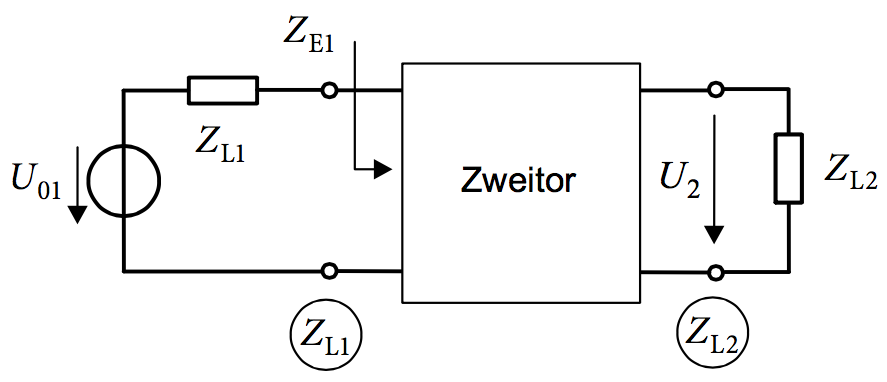
\includegraphics[width=0.5\linewidth]{img/streuparameter}

Reflexions- und Transmissionsfaktoren
	\begin{equation*}
		\c{S}_{ii}=\frac{\c{Z}_{\text{E}i}-\c{Z}_{\text{L}i}}{\c{Z}_{\text{E}i}+\c{Z}_{\text{L}i}} \qquad \c{S}_{ji}=2\frac{\c{U}_j}{\c{U}_{0i}}\sqrt{\frac{\c{Z}_{\text{L}i}}{\c{Z}_{\text{L}j}}} \qquad \parbox{0.4\linewidth}{Statt Einzelspannungen Spannungsteiler einsetzen. Auf Parallelschaltungen Achten)}
	\end{equation*}
Serienimpedanz  und Paralleladmittanz
	\begin{equation*}
		\c{\matr{S}}_{^{-}}=\frac{1}{\c{Z}+2R_\text{N}}
		\begin{pmatrix}
			\c{Z} & 2R_\text{N}\\
			2R_\text{N} & \c{Z}
		\end{pmatrix}
		\qquad
		\c{\matr{S}}_{||}=\frac{1}{2+\c{Y}R_\text{N}}
		\begin{pmatrix}
			-\c{Y}R_\text{N} & 2\\
			2 & -\c{Y}R_\text{N}
		\end{pmatrix}
	\end{equation*}
\subsection{Zusammenhang Impedanz-, Admittanz- und Streumatrix}
	\begin{align*}
		\c{\matr{S}}&=\matr{E}-2R_\text{N}(\c{\matr{Z}}+R_\text{N}\matr{E})^{-1} & \c{\matr{Z}}&=-R_\text{N}(\matr{E}+2(\c{\matr{S}}-\matr{E})^{-1})\\
		&=-\matr{E}+2(R_\text{N}\c{\matr{Y}}+\matr{E})^{-1} & \c{\matr{Y}}&=-\frac{1}{R_\text{N}}(\matr{E}-2(\c{\matr{S}}+\matr{E})^{-1})
	\end{align*}
\HL
\section{Smith-Diagramme}
\subsection{Ablesen und Antragen der Werte}
	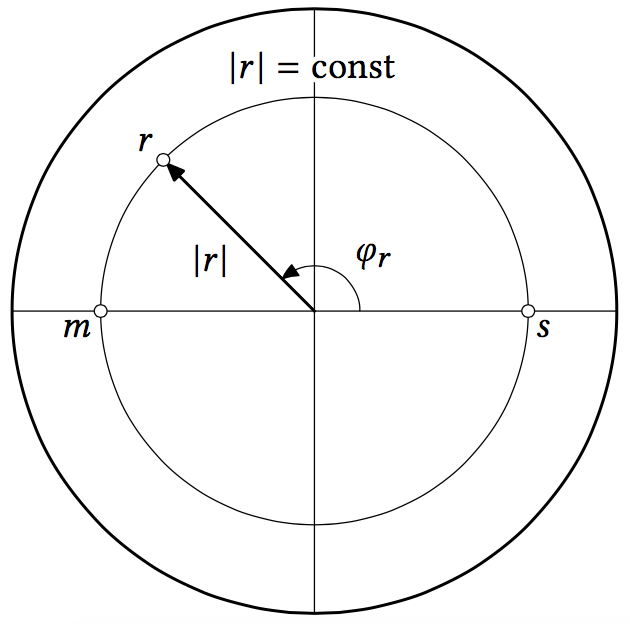
\includegraphics[width=0.45\linewidth]{img/rzsm}
	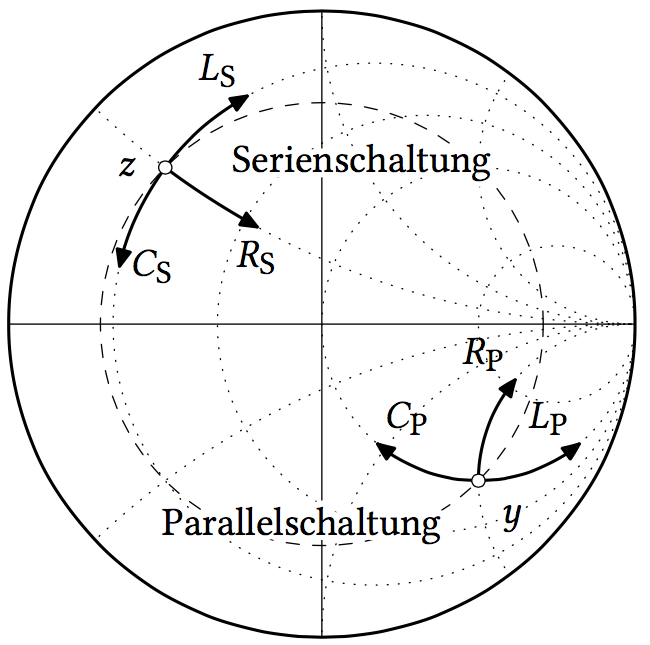
\includegraphics[width=0.45\linewidth]{img/bauelemente}
	\begin{equation*}
		|\c{\Gamma}|=r=\frac{\c{Z}-\c{Z_L}}{\c{Z}+\c{Z}_L}=\frac{\c{z}-1}{\c{z}+1}=\frac{s-1}{s+1}=\frac{1-m}{1+m}\qquad s=\frac{1}{m}=\frac{1+|r|}{1-|r|}
	\end{equation*}
\HL
\section{Allgemeines}
	\begin{equation*}
		\si{\decibel}=10\log(\dots) \qquad \si{\decibel}_\text{m}=10\log\left(\frac{P}{\SI{1}{\milli\watt}}\right)
	\end{equation*}
\subsection{Additionstheoreme}
		\begin{align*}
			\cos^2(\alpha)&=\frac{1}{2}(1+\cos(2\alpha))\\
			\sin^2(\alpha)&=\frac{1}{2}(1-\cos(2\alpha))\\
			\sin(\alpha)\cos(\beta)&=\frac{1}{2	}(\sin(\alpha-\beta)+\sin(\alpha+\beta))
		\end{align*}
\subsection{SI-Präfixe}
\begin{tabular}{|l|l|l||l|l|l|}
\hline
\textbf{Präfix} & \textbf{Zeichen} & \textbf{Faktor} & \textbf{Präfix} & \textbf{Zeichen} & \textbf{Faktor}\\
\hline\hline
Yocto  & y  & $10^{-24}$ & Deka   & da & $10^{1}$\\
\hline
Zepto  & z  & $10^{-21}$ & Hekto  & h  & $10^{2}$\\
\hline
Atto   & a  & $10^{-18}$ & Kilo   & k  & $10^{3}$\\
\hline
Femto  & f  & $10^{-15}$ & Mega   & M  & $10^{6}$\\
\hline
Piko   & p  & $10^{-12}$ & Giga   & G  & $10^{9}$\\
\hline
Nano   & n  & $10^{-9}$ & Tera   & T  & $10^{12}$\\
\hline
Mikro  & $\mu$ & $10^{-6}$ & Peta   & P  & $10^{15}$\\
\hline
Milli  & m  & $10^{-3}$ & Exa    & E  & $10^{18}$\\
\hline
Zenti  & c  & $10^{-2}$ & Zetta  & Z  & $10^{21}$\\
\hline
Dezi   & d  & $10^{-1}$ & Yotta  & Y  & $10^{24}$\\
\hline
\end{tabular}
\vfill
\HL\\
\shorthandoff{"}
zusammengestellt von \textsc{Tino Steinmetz} und \textsc{Hermann Pommerenke},\\ basierend auf der Vorlesung "Hochfrequenztechnik" von \textsc{Prof. Tobias Weber}\\ \textsc{Universität Rostock}, SS 2015
\end{multicols}	

\end{document}
